\section{RL}
Idea: Model world as MDP, but we don't know $T$ and $R$.

\textbf{Model-Based RL}
Approximate $T$ and $R$ based on experiences. Average $R$ and $T$ across epsiodes.
\begin{figure}[H]
    \centering
    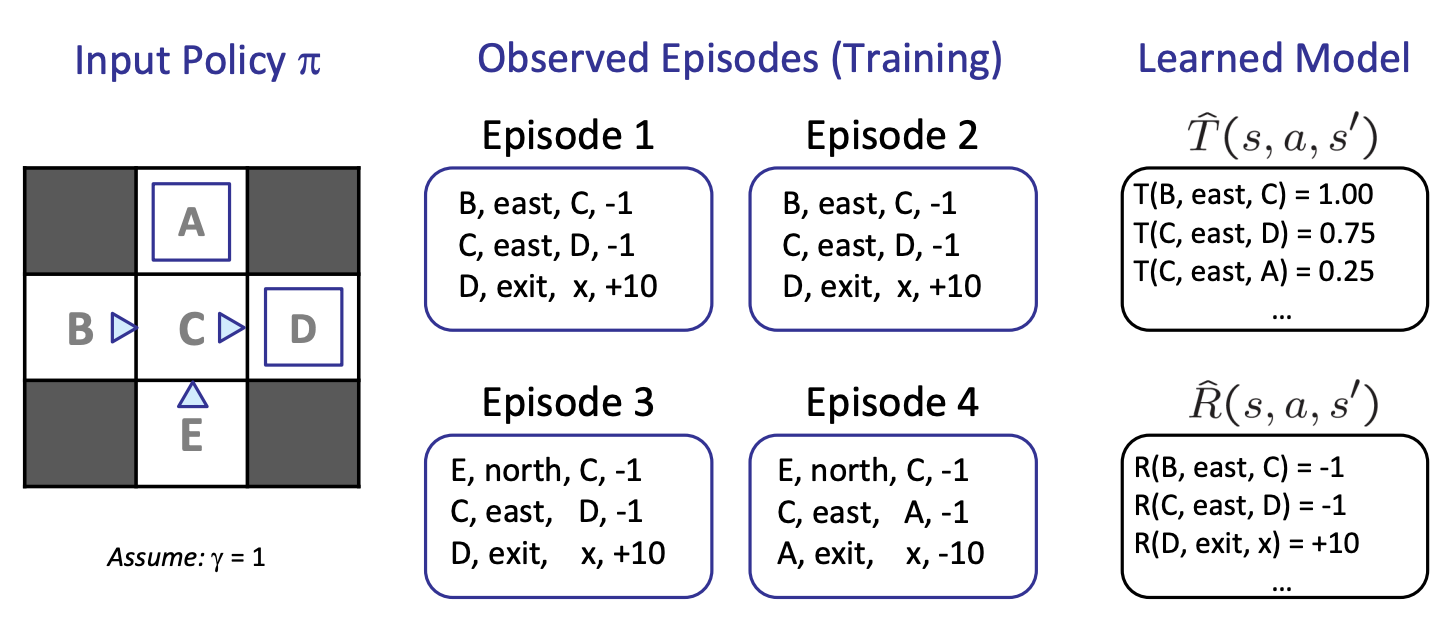
\includegraphics[width=\linewidth]{model-based}
\end{figure}
\textbf{Model-Free RL}

\textbf{Direct Evaluation:} Learn values of states from episodes.
\begin{figure}[H]
    \centering
    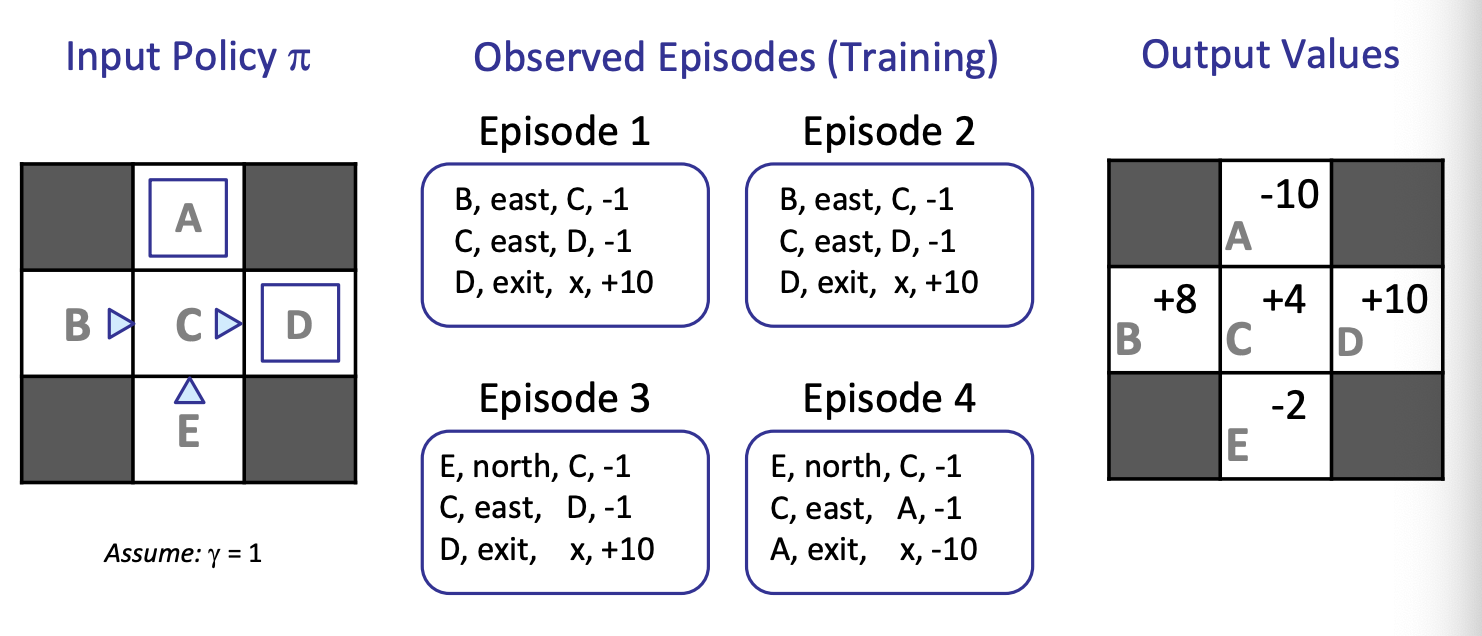
\includegraphics[width=\linewidth]{direct-evaluation}
\end{figure}


Assuming $\gamma = 1$:

$E1: V(D) = 10, V(C) = 9, V(B) = 8$

$E2: V(D) = 10, V(C) = 9, V(B) = 8$

$E3: V(D) = 10, V(C) = 9, V(E) = 8$

$E4: V(D) = -10, V(C) = -11, V(B) = -12$

Values of each state are averaged across episodes. Wastes information about state connections.

\textbf{TD-Learning:} Fix $\pi$, learn $V$ of states at the transition level, not episodes.

$sample = R + \gamma V(S')$

$V^{\pi}(S) \leftarrow (1 - \alpha) * V^{\pi}(S) + \alpha * sample$

But we can't directly extract a policy since we don't know transition prob. $T$ of actions $a$, so we apply this idea to $Q$-values instead.

\textbf{$Q$-learning:} Don't need to fix $\pi$ since we are learning $Q$-values.

$sample = R(s, a, s') + \gamma * \max_{a'} Q(s', a')$

$Q(s, a) \leftarrow (1 - \alpha) * Q(s, a) + \alpha * sample$

\textbf{Exploration:} need to explore to learn optimal policy.

$\epsilon$-greedy policy: $\pi(s) = \text{argmax}_a Q(s, a)$ with probability $1 - \epsilon$, otherwise pick random action.

Keep track of visit counts $N(s, a)$ and use a modified $Q$-value function:

$f(u, n) = u + k / n$

$Q(s, a) \leftarrow (1 - \alpha) * Q(s, a) + \alpha * (R + \gamma * \max_{a'} f(Q(s', a'), N(s', a'))$

Softmax Exploration: $\tau$ controls how greedy / random we are.

$\pi(s | a) = \frac{e^{Q(s, a) / \tau}}{\sum_{a'} e^{Q(s, a') / \tau}}$

\textbf{Approximate Q-Learning:} To not have to learn $Q$ for all states, find $Q$ for a set of features $f(s, a)$ by learning weights $w$.

$Q(s, a) = w^T f(s, a)$

$\text{difference} = (R + \gamma * \max_{a'} Q(s', a')) - w^T f(s, a)$. Note: the left term is a fixed target.

$L(w) = \frac{1}{2}(\text{difference})^2$

$w_i \leftarrow w_i - \nabla L(w) = w_i + \alpha * f_i(s, a) * \text{difference}$

Minimizing error via gradient descent.






